\documentclass{book}
%\usepackage[a4paper]{geometry}
\usepackage{graphicx}
\usepackage{color}
\usepackage{url}
\usepackage{amssymb}
\usepackage{amsmath}
\usepackage{hyperref}
%\usepackage{xcolor}
\usepackage{epstopdf}
\usepackage{rotating}
\usepackage[dvipsnames]{xcolor}
\usepackage{listings}
\usepackage{color}
\usepackage{fontspec}	% To change default font
%\usepackage{courier}

\definecolor{mygreen}{rgb}{0,0.6,0}
\definecolor{mygray}{rgb}{0.5,0.5,0.5}
\definecolor{mymauve}{rgb}{0.58,0,0.82}
\definecolor{dark-red}{rgb}{0.4,0.15,0.15}
\definecolor{dark-blue}{rgb}{0.15,0.15,0.8}
\definecolor{medium-blue}{rgb}{0,0,0.5}
\definecolor{backcolour}{rgb}{0.95,0.95,0.92}

\hypersetup{colorlinks, linkcolor={dark-blue},
    citecolor={dark-blue}, urlcolor={medium-blue}} % For hyperlinks

\lstset{ 
  backgroundcolor=\color{backcolour},   % choose the background color; you must add \usepackage{color} or \usepackage{xcolor}
  basicstyle=\ttfamily,		% the size and type of the fonts that are used for the code
  numbers=left ,				% where to put the line-numbers
  numberstyle=\footnotesize, % size of the fonts used for the line-numbers
  stepnumber=1, % the step between two line-numbers.
  numbersep=5pt, % how far the line-numbers are from the code
  breakatwhitespace=false,         % sets if automatic breaks should only happen at whitespace
  breaklines=true,                 % sets automatic line breaking
  captionpos=t,                    % sets the caption-position to bottom
  showstringspaces=false
  frame=single,	                 % adds a frame around the code
  commentstyle=\color{mygreen},    % comment style
  keywordstyle=\color{blue},       % keyword style
  numberstyle=\tiny\color{mygray}, % the style that is used for the line-numbers
  stringstyle=\color{mymauve},     % string literal style
  language=Scilab,                 % the language of the code
  title=\lstname                   % show the filename of files included with \lstinputlisting; also try caption instead of title
}

\usepackage{appendix}
%\usepackage{wrapfig}
%\usepackage{lscape}
\usepackage{rotating} % for rotaing figure sideways

%\usepackage{fancyhdr}	%to include customized footer and header
%\pagestyle{fancy}
%\lhead{}
%\chead{\leftmark}
\graphicspath{{./Figures/}}
%\setmainfont{URW Palladio L} % Use if font is to be set

\begin{document}
%-----------------------------------
% For customised Title Page
\thispagestyle{empty}
%\input{./title.tex} %Cover page
\thispagestyle{empty}
%\input{./inner.tex}	%Inner title page
%--------------------------------------------------------------------

%Default Title page 
\title{DC and DSP Lab using Scilab}
%\date{December 2013}
\author{Kavya Manohar} {%Authors: Kavya Manohar}
\maketitle
%----------------------------------------------------------
%\thispagestyle{empty}
  
\noindent \textcopyright{}2016, Kavya Manohar.\\
\noindent
This work is licensed under a Creative Commons Attribution-Share Alike 4.0 India License. See \url{http://creativecommons.org/licenses/by-sa/4.0/} for more details.
\\[5cm]

\noindent \textbf{This is a laboratory manual for DC and DSP simulation laboratory. It mostly adheres to the syllabus of the  University of Calicut.}
\\

%\noindent This project is hosted at:  \url{https://github.com/kavyamanohar/analogcommunication}


\noindent Contact: sakhi.kavya@gmail.com

%------------------------------------------------------------

\clearpage
\thispagestyle{plain}
%\par\vspace*{.35\textheight}{\centering Dedicated to my parents\par}  % code for dedication page
\chapter*{Preface} 

This laboratory manual has been prepared to aid the students in carrying out some basic experiments in Digital Communication and Digital Signal Processing using Scilab. It is assumed that the student has some basic understanding on the programming environemnt of Scilab. If not go through some tutorials listed in the reference section.

Each chapter contains basic theory regarding the experiment. The scilab code to carryout the experiment and the resulting plot and figures are also included as subsection. 

This is a work in progress version of the laboratory manual. Suggestions on improvement in conceptual clarity, diagrams, typography are most welcome. Share whatever you feel about the book- it is yours.

\begin{flushright}
\textbf{Kavya Manohar}
\end{flushright}
\chapter*{Acknowledgements}

Thank you for going through this work. Thanks in advance for your valuable feedbacks that would help improve this book.

Thanks a lot for the lectures and notes of Prof. Madhavan Nair, Retired Professor, College of Engineering Trivandrum, which helped me to draft this manual.

Thanks to my colleagues at Aryanet Institute of Technology for their encouragement and support. Special thanks to Sathyan P. for being with me experimenting in the laboratory. Thanks to my students who helped me improve the contents with timely comments.

Thanks to all free knowledge enthusiasts- especially to those who have created and shared electronics and communication engineering related contents to various public domain sources. Your efforts have helped a lot in the making of this book.

Thanks Santhosh, for what you are to me.

\begin{flushright}
\textbf{Kavya Manohar}
\end{flushright}







\thispagestyle{empty}
\tableofcontents
\thispagestyle{empty}
\thispagestyle{empty}

\listoffigures
\thispagestyle{empty}
%CHAPTER-----------------------------------------------------------------------

\chapter [Introduction to Scilab]{Introduction to Scilab}


\section{AIM}
\begin{itemize}
\item
Study of SCILAB basics and getting familiar with the environment.
\item
Generation of various waveforms in continuous and discrete form.
\begin{itemize}
\item
Unit impulse signal
\item
Unit step signal
\item
Unit ramp signal
\item
Triangular signal
\item

Exponential signal
\item
Sinusoidal signal
\end{itemize}
\end{itemize}

\section{THEORY}
\paragraph{}

Scilab is an open source software for numerical mathematics and scientific visualization. It is capable of interactive calculations as well as automation of computations through programming. It provides all basic operations on matrices through built-in functions so that the trouble of developing and testing code for basic operations are completely avoided. Its ability to plot 2D and 3D graphs helps in visualizing the data we work with. All these make Scilab an excellent tool for teaching, especially those subjects that involve matrix operations. Further, the numerous toolboxes that are available for various specialized applications make it an important tool for research. Being compatible with Matlab®, all available Matlab M-files can be directly used in Scilab with the help of the Matlab to Scilab translator.Scicos, a hybrid dynamic systems modeler and simulator for Scilab, simplifies simulations. The greatest features of Scilab are that it is multiplatform and is free. It is available for many operating systems including Windows, Linux and MacOS X. \cite{scilab}
\paragraph{}

Scilab is a scientific software package which was developed since 1990 by researchers from INRIA(French National Institute for Research in Computer Science and Control) andENPC (National School of Bridges and Roads), it is now maintained anddeveloped by ScilabConsortium since its creation in May 2003 and integrated into Digiteo Foundation in July 2008. The current version is 5.5.1 (February2010).Since 1994 it is distributed freely along with source code through the Internet and is currently being used in educational and industrial environments around the world. From version 5 it is released under the GPL compatible CeCILL license.
\paragraph{}

When you start up Scilab, you see a window called Scilab console. The user enters Scilab commands at the prompt (-->). But many of thecommands are also availablethrough the menu at the top. Themost important menu for abeginner is the “Help” menu.Clicking on the “Help” menu opensup the Help Browser, showing alist of topics on which help isavailable. Clicking on the relevanttopic takes you to hyperlinkeddocuments similar to web pages. The codes for the programs are written as SciNotes by selecting a blank note from the tope top left corner of the Scilab Console.

\section{PROCEDURE}

\paragraph{}
\begin{enumerate}
\item
Start Scilab on PC and Scilab console window opens. Create a new blank SciNote.
\item
The code for the required program is typed and saved as Scilab SCE file with an extension .sci
\item

The continuous plots are made using the function “plot” and discrete plots are made using the function “plot2d3” with the corresponding x axis and y axis variables written inside().

\item
To view all the plots in the same window the function “subplot” is used.
\item
The results and the errors in the program are displayed in the console window.
The typed program is run using the “execute”.
\end{enumerate}

\section{SCILAB CODE}
\subsection*{Operations on discrete signals}


\lstinputlisting[title='Discrete Signals']{./scilabCode/discretesignals.sci}

\subsection*{Operations on continuous signals}
%\VerbatimInput{./continuoussignals.sci}


\chapter [Basic Signal Operations]{Basic Signal Operations}


\section{AIM}
\begin{enumerate}
\item
For a given signal generate its
\begin{itemize}
\item
Folded signal sequence
\item
Time delayed and advanced sequences

\end{itemize}
\item
For the given two signals in discrete domain perform signal addition and subtraction
\item
Perform linear convolution on given two sequences..

\end{enumerate}
\section{THEORY}
\paragraph{}

The time reversal of a discrete time signal $x(n)$ can be obtained by folding the sequence about $n=0$ and the folded sequence is represented by $x(-n)$. The signal time delayed by 3 samples  is obtained by shifting the sequence to right by 3 samples and it is represented with $x(n-3)$. The signal time advanced by 2 samples  is obtained by shifting the sequence to left by 2 samples and it is represented with $x(n+2)$.	
	
	
	For discrete-time signals the sum of two sequences and difference of two sequences is obtained by adding and subtracting the sequence values at the same index $n$ for which the sequences are defined.
	
The convolution between the input sequence $x(n)$ and impulse response $h(n)$ is computed using the function $convol$ as $y=convol(x,h)$. If the length of $x(n)$ is $N_1$ and length of $h(n)$ is $N_2$ , then the length of $y(n)$ is $N_1+N_2-1$. The length of $x(n)$ and $h(n)$ is found using the function $length(x)$ and $length(h)$ . If the sequence $x(n)$ is starting at $n_1$ and $h(n)$ at $n_2$, then sequence $y(n)$ starts at $n_1+n_2$.

\section{PROCEDURE}

\paragraph{}
\begin{enumerate}
\item
Start Scilab on PC and Scilab console window opens. Create a new blank SciNote.
\item
The code for the required program is typed and saved as Scilab SCE file with an extension .sci
\item

The continuous plots are made using the function $plot$ and discrete plots are made using the function $plot2d3$ with the corresponding x axis and y axis variables written inside parathesis.

\item
To view all the plots in the same window the function $subplot$ is used.
\item
The results and the errors in the program are displayed in the console window.
The typed program is run using the $execute$.
\item
The resultant figure is exported as pdf using $xs2pdf$
\end{enumerate}

\section{SCILAB CODE}

\lstinputlisting[caption=Scilab code for a folded sequence]{./scilabCode/folded_sequence.sci}

\lstinputlisting[caption=Scilab code for sequences with time shifted versions]{./scilabCode/timeshift.sci}



\lstinputlisting[caption=Addition and Subtraction of signals]{./scilabCode/add_subtract.sci}



\lstinputlisting[caption=Linear Convolution]{./scilabCode/linearconvolution.sci}




\section{RESULT}
Different signal operations were performed using SCILAB.
\begin{figure}
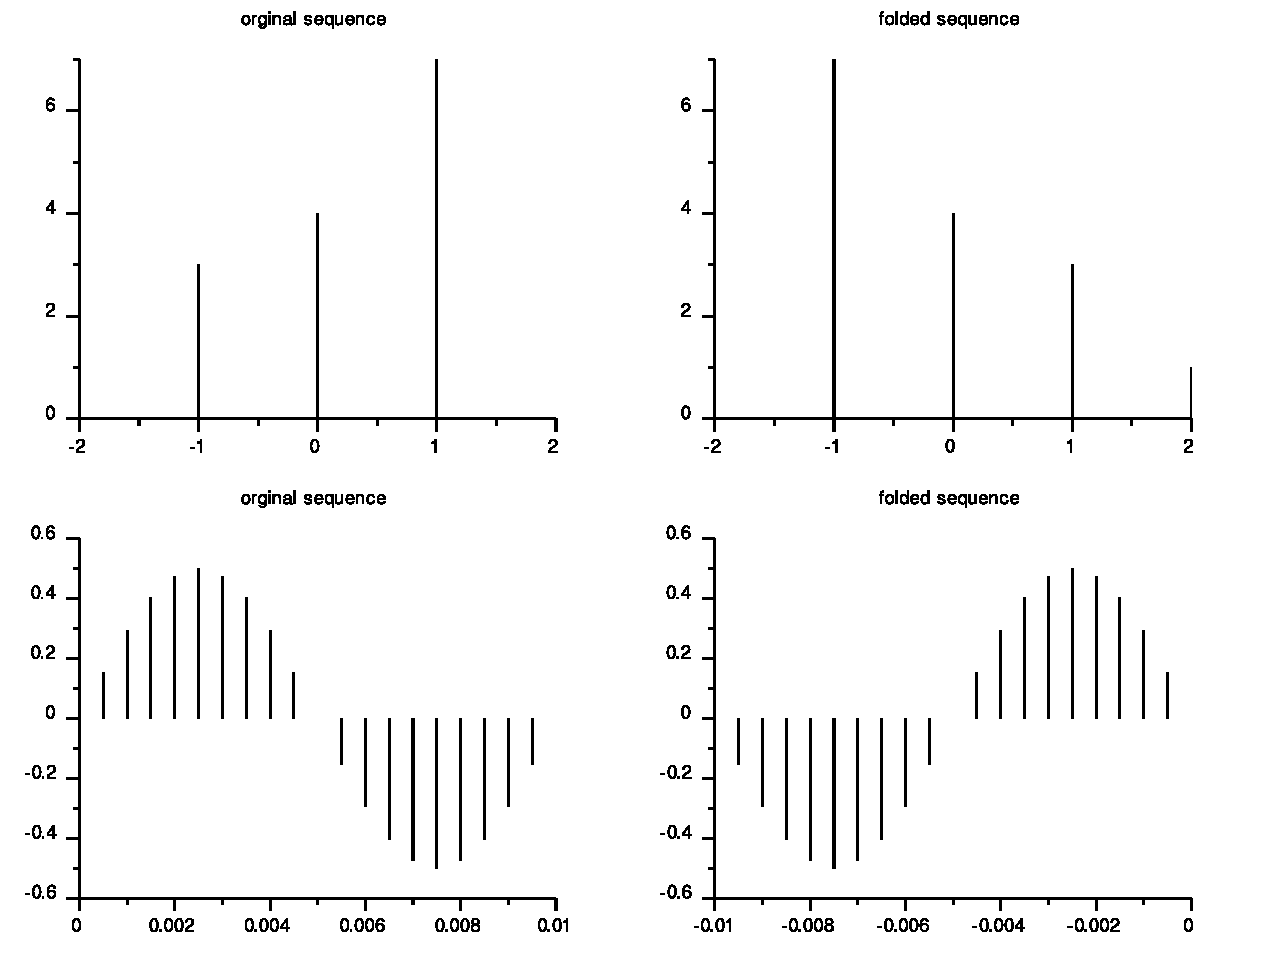
\includegraphics[scale=.5]{/home/kavya/kavyadev/DSPlab/scilabCode/foldedsequence.pdf}
\caption{Plot of signals and their folded versions}
\label{folded}
\end{figure}

\begin{figure}
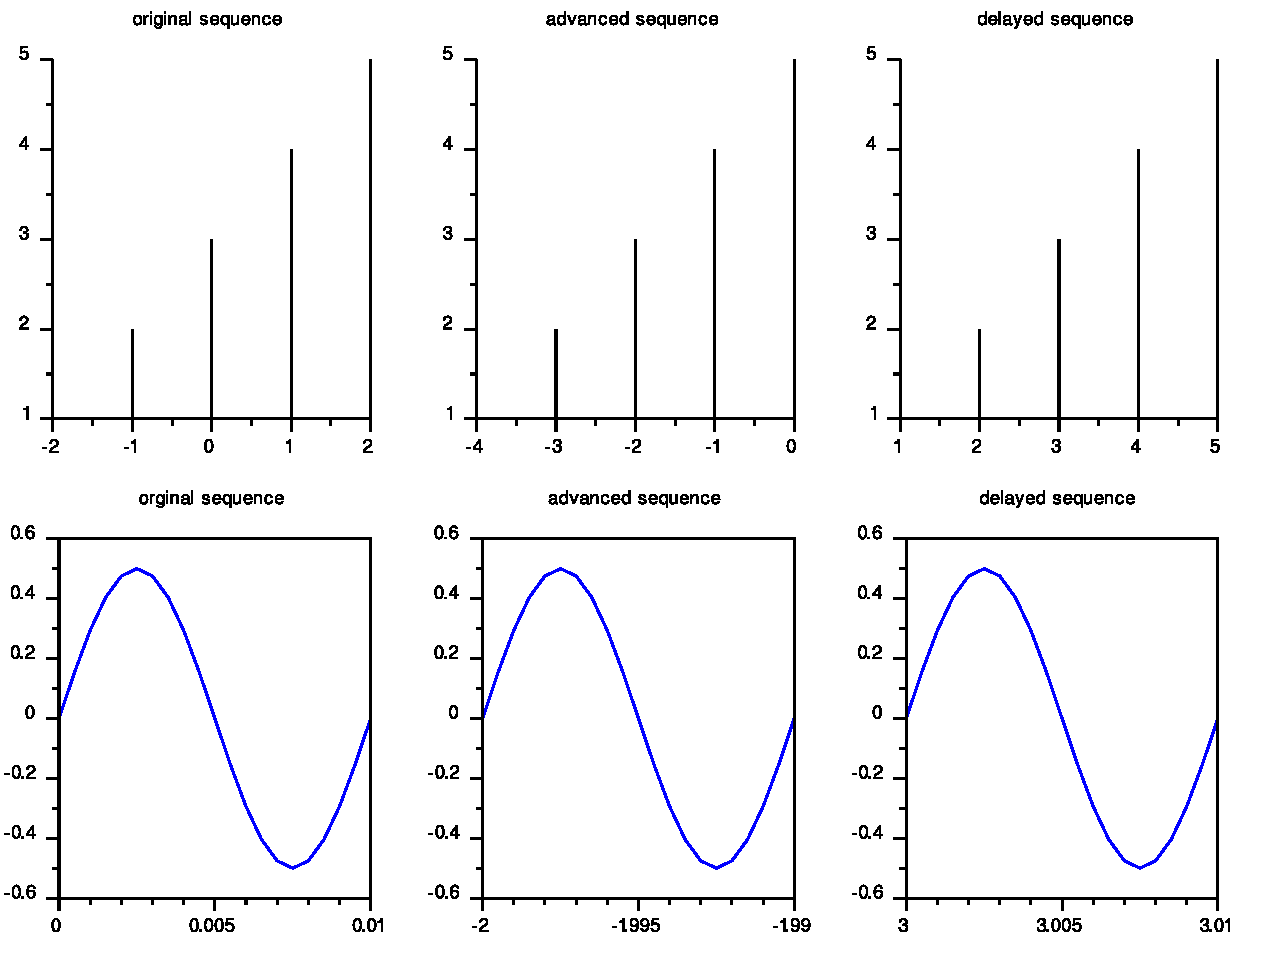
\includegraphics[scale=.5]{/home/kavya/kavyadev/DSPlab/scilabCode/timeshift.pdf}
\caption{Plot of signals and their shifted versions}
\label{shifted}
\end{figure}


\begin{figure}
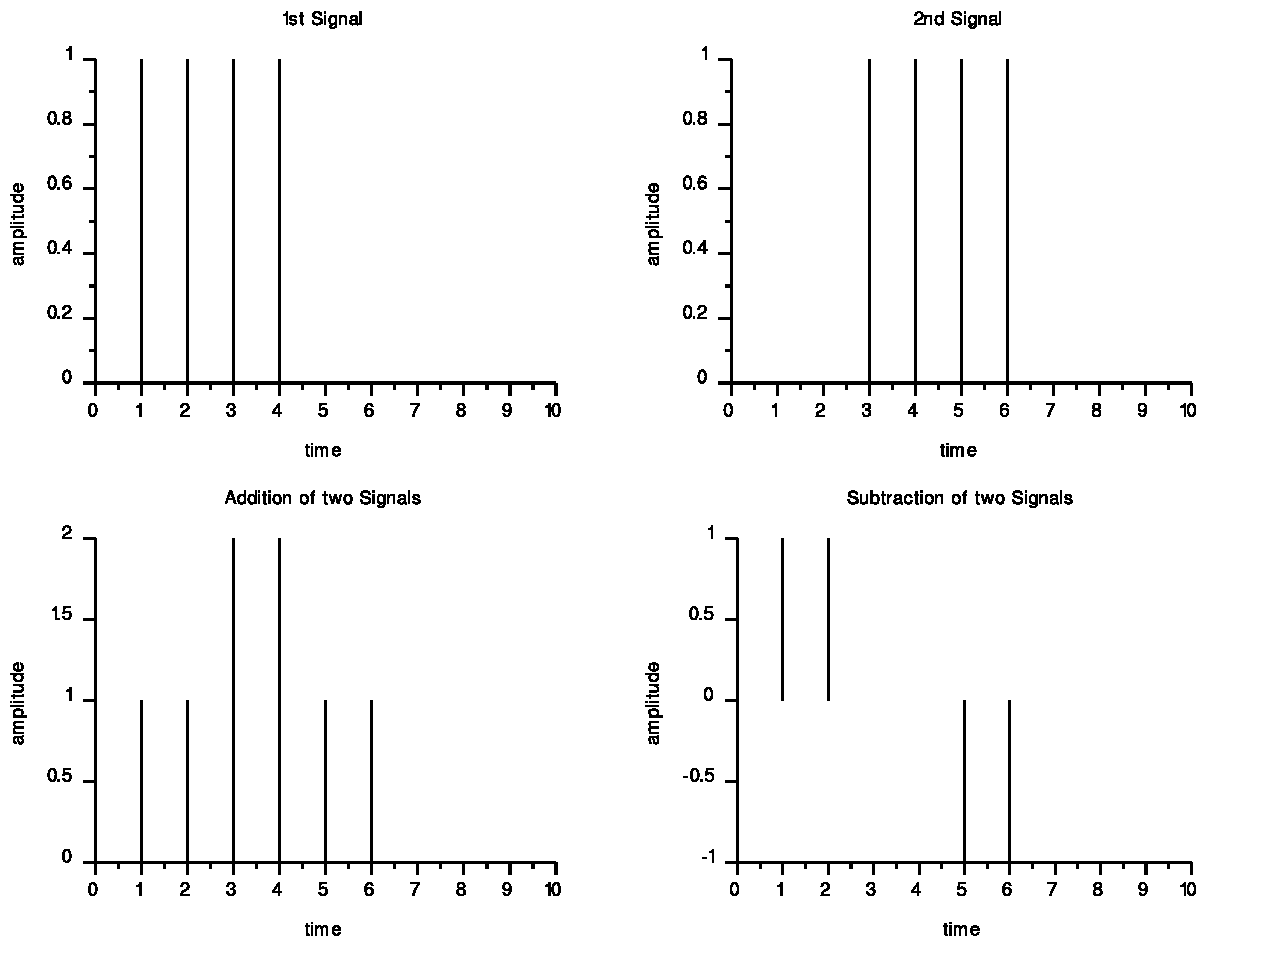
\includegraphics[scale=.5]{/home/kavya/kavyadev/DSPlab/scilabCode/addSubtract.pdf}
\caption{Plot of signals, their sum and their difference}
\label{addSub}
\end{figure}

\begin{figure}
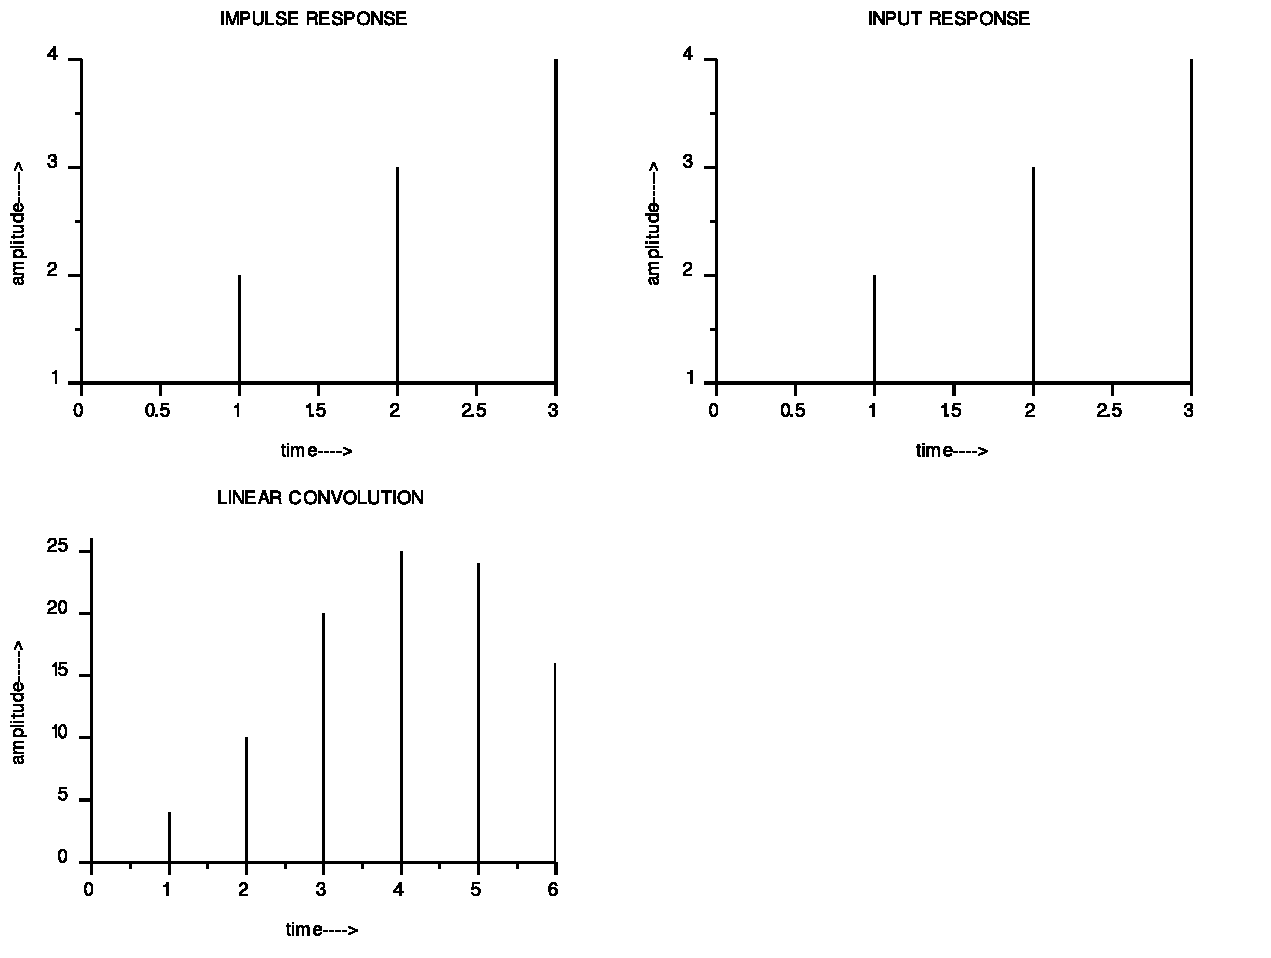
\includegraphics[scale=.5]{/home/kavya/kavyadev/DSPlab/scilabCode/linearconvolution.pdf}
\caption{Linear convolution of two sequences}
\label{linconv}
\end{figure}



\chapter [Discrete Fourier Transform]{Discrete Fourier Transform}


\section{AIM}
\begin{enumerate}
\item
Generate the sum of two sinewaves and analyse their spectrum.
\item
Find the DFT of given sequence and plot it.

\item
Find the circular convolution of two sequences.


\end{enumerate}
\section{THEORY}
\paragraph{}

Discrete fourier transform is found using the function fft(x,-1) and inverse discrete fourier transform using fft(x,1). To plot the magnitude and phase response, magnitude is found using the function abs(x) and phase using the function atan(imag(x),real(x)) .To find circular convolution of two signals x1(n) and x2(n) their corresponding dfts are found and multiplied to get Y(K)= X1(K)*X2(K).  IDFT of Y(K) gives y(n). To find circular convolution of two sequences both the sequences must be of same length and if not zeros are added to smallest sequence. 
\section{PROCEDURE}

\paragraph{}
\begin{enumerate}
\item
Start Scilab on PC and Scilab console window opens. Create a new blank SciNote.
\item
The code for the required program is typed and saved as Scilab SCE file with an extension .sci
\item

The continuous plots are made using the function $plot$ and discrete plots are made using the function $plot2d3$ with the corresponding $x$ axis and $y$ axis variables written inside paranthesis.

\item
To view all the plots in the same window the function $subplot$ is used.
\item
The results and the errors in the program are displayed in the console window.
The typed program is run using the $execute$.
\end{enumerate}

\section{SCILAB CODE}
\subsection{Frequency content of a sine wave}
\lstinputlisting[caption=Scilab code for finding frequency content in the sum of two sine waves]{./scilabCode/sine_dft.sci}



\subsection{DFT of a sequence}
\lstinputlisting[caption=Scilab code for finding frequency content in a sequence]{./scilabCode/dft_sequence.sci}


\subsection{Circular convolution using DFT}
\lstinputlisting[caption=Scilab code for finding circular confolution using dft]{./scilabCode/circular_conv.sci}


\section{RESULT}
Different signal operations were performed using SCILAB.
\begin{figure}
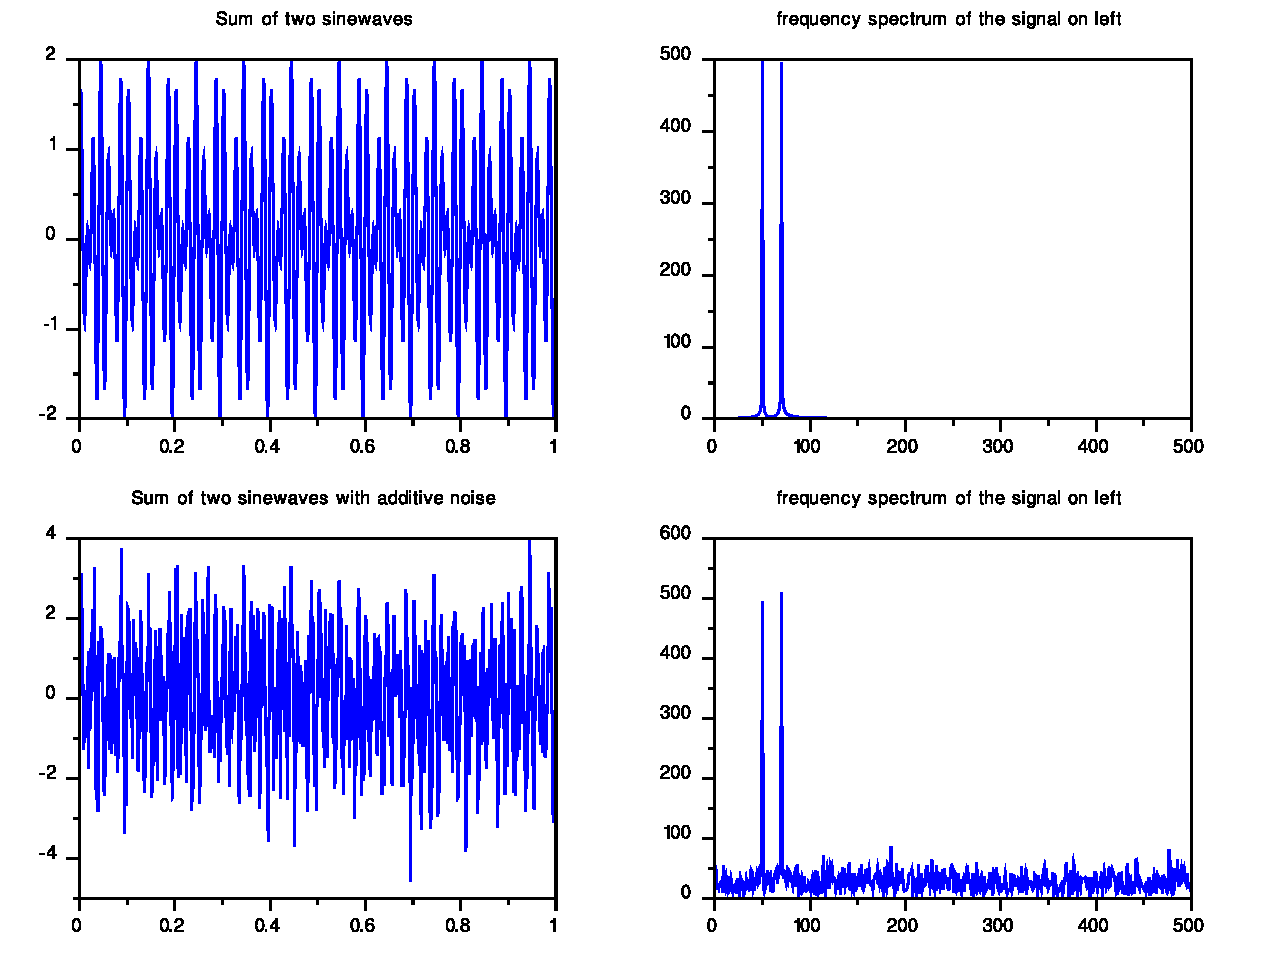
\includegraphics[scale=.5]{/home/kavya/kavyadev/DSPlab/scilabCode/sine_dft.pdf}
\caption{Plot of pure and noisy sine waves and their discrete Fouruer Transform}
\label{sine_dft}
\end{figure}

\begin{figure}
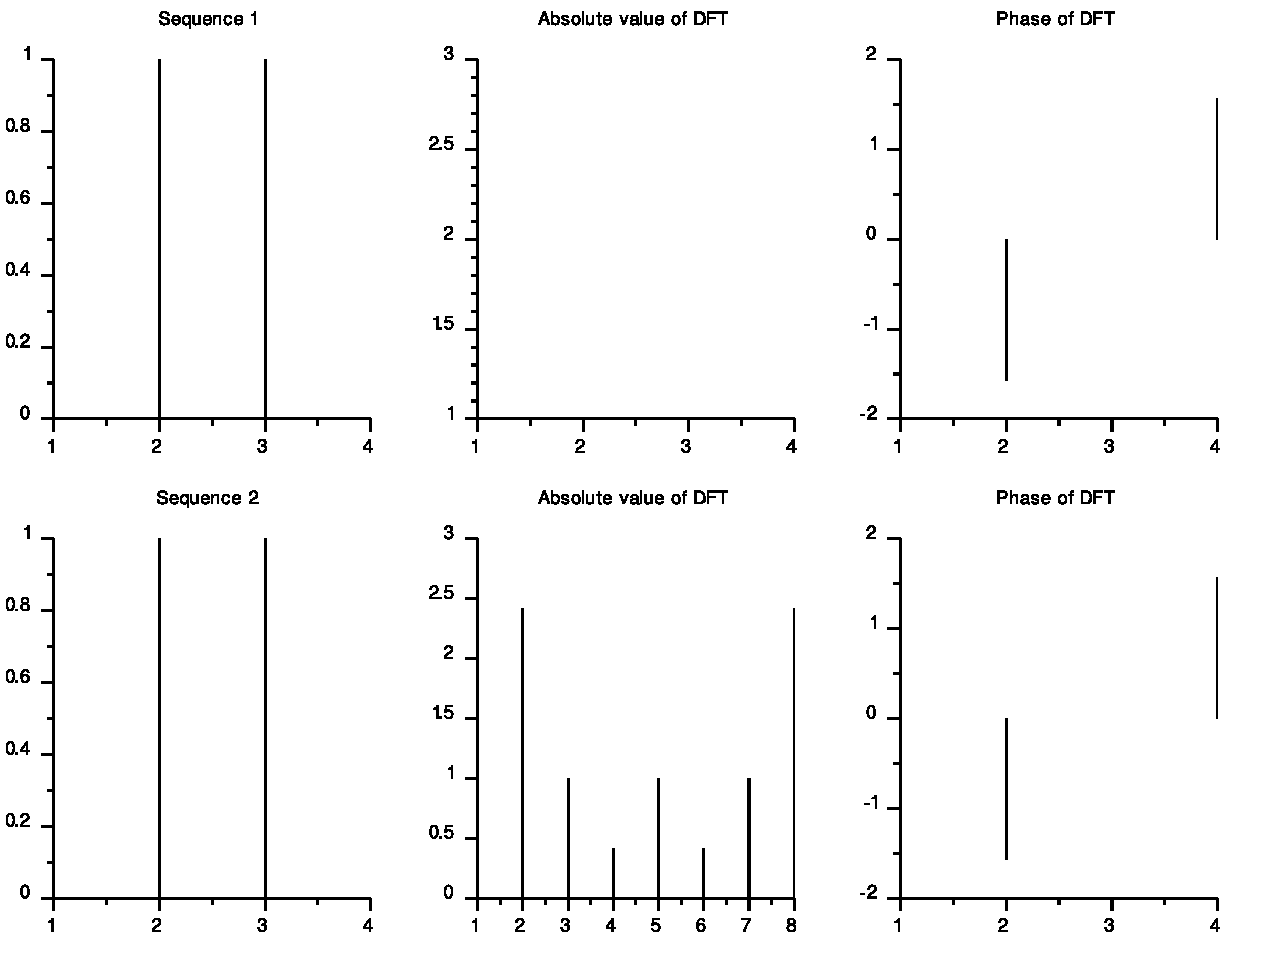
\includegraphics[scale=.5]{/home/kavya/kavyadev/DSPlab/scilabCode/dft_sequence.pdf}
\caption{Plot of a sequence and its DFT(magnitude and phase)}
\label{dft_sequence}
\end{figure}

\begin{figure}
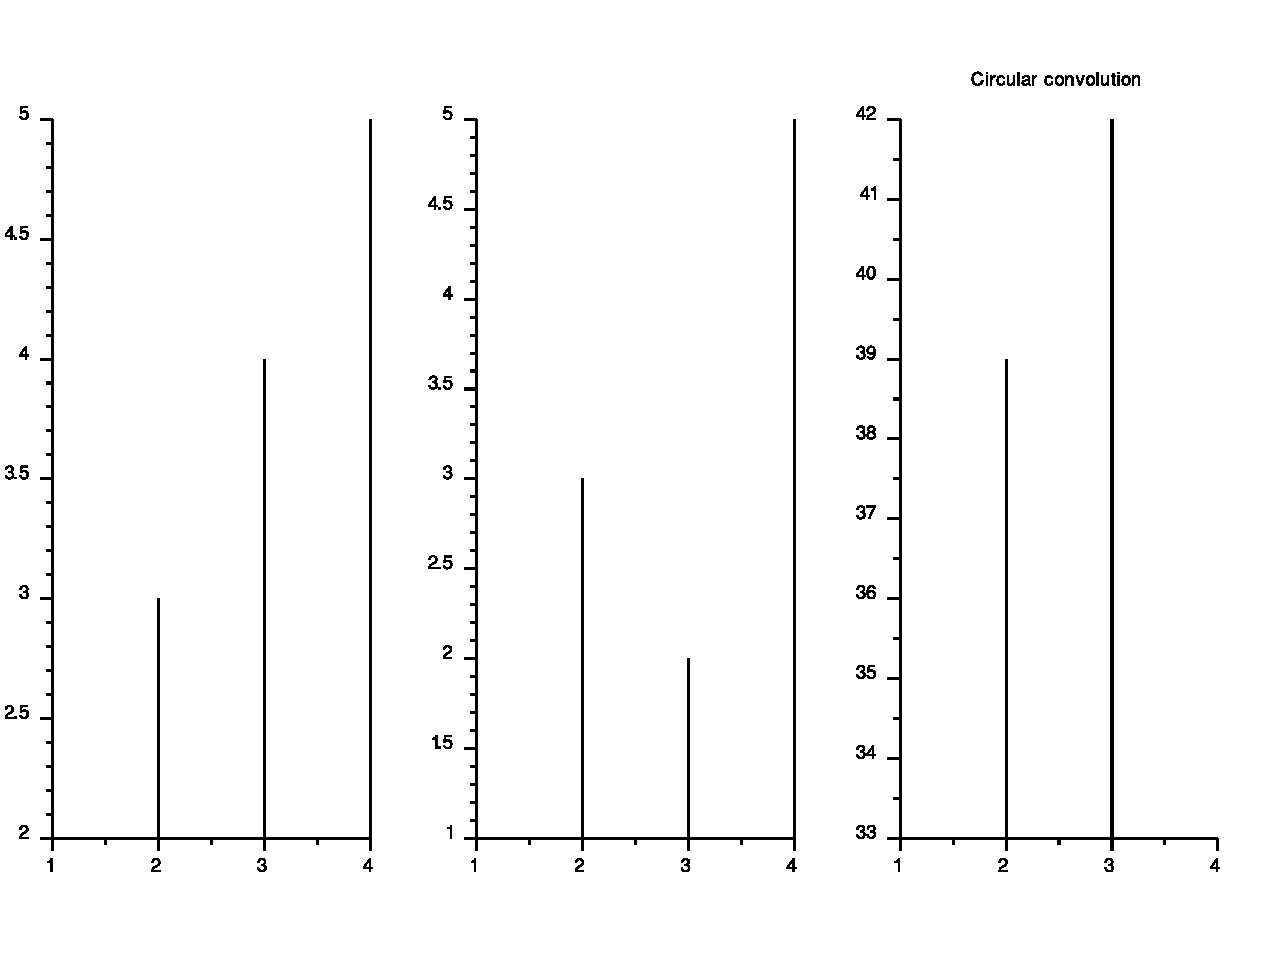
\includegraphics[scale=.5]{/home/kavya/kavyadev/DSPlab/scilabCode/circular_conv.pdf}
\caption{Plot of a sequence and its circular convolution}
\label{circular_conv}
\end{figure}
\chapter [Performance Comparison of Modulation Scheme]{Performance Evaluation of Modulation Scheme}


\section{AIM}

Implement a digital modulation scheme (BASK and BPSK) using Scilab. Add noise of different SNR level to model a transmission channel. Demodulate it and find BER for each case and plot it. Compare it with theoretical model.


\section{THEORY}

Digital data with binary values are modulated and represented as the binary phase of a sinusoidal carrier in BPSK signalling scheme. The decoding will be erroneous if additive noise disrupts the modulated signal during transmission. The bit error rate (BER) decreases with increase in Signal to Noise Ratio (SNR). 

The following experiment compares the theoretical relation between the two with simulated values of BER. Noise corresponding to different values of SNR is added to the modulated signal and the resulting signal is used for message detection. The demodulated message is then compared with the actual message to find the BER corresponding to each value of SNR(2 dB, 4 dB, 6 dB, 8 dB, 10 dB).

\section{PROCEDURE}

\paragraph{}
\begin{enumerate}
\item
Start Scilab on PC and Scilab console window opens. Create a new blank SciNote.
\item
The code for the required program is typed and saved as Scilab SCE file with an extension .sci
\item

The continuous plots are made using the function $plot$ and discrete plots are made using the function $plot2d3$ with the corresponding x axis and y axis variables written inside().

\item
To view all the plots in the same window the function “subplot” is used.
\item
The results and the errors in the program are displayed in the console window.
The typed program is run using the “execute”.
\end{enumerate}

\section{SCILAB CODE}
%\subsection*{Comparison of BER performance for different SNR levels for BASK}
%\VerbatimInput{./berevaluation.sci}
\subsection*{Comparison of BER performance for different SNR levels for BPSK}
\lstinputlisting[caption=Comparison of BER performance for different SNR levels for BPSK]{./scilabCode/berbpsk.sci}



\section{RESULT}
Performance evaluation plots were implemented.

\begin{figure}
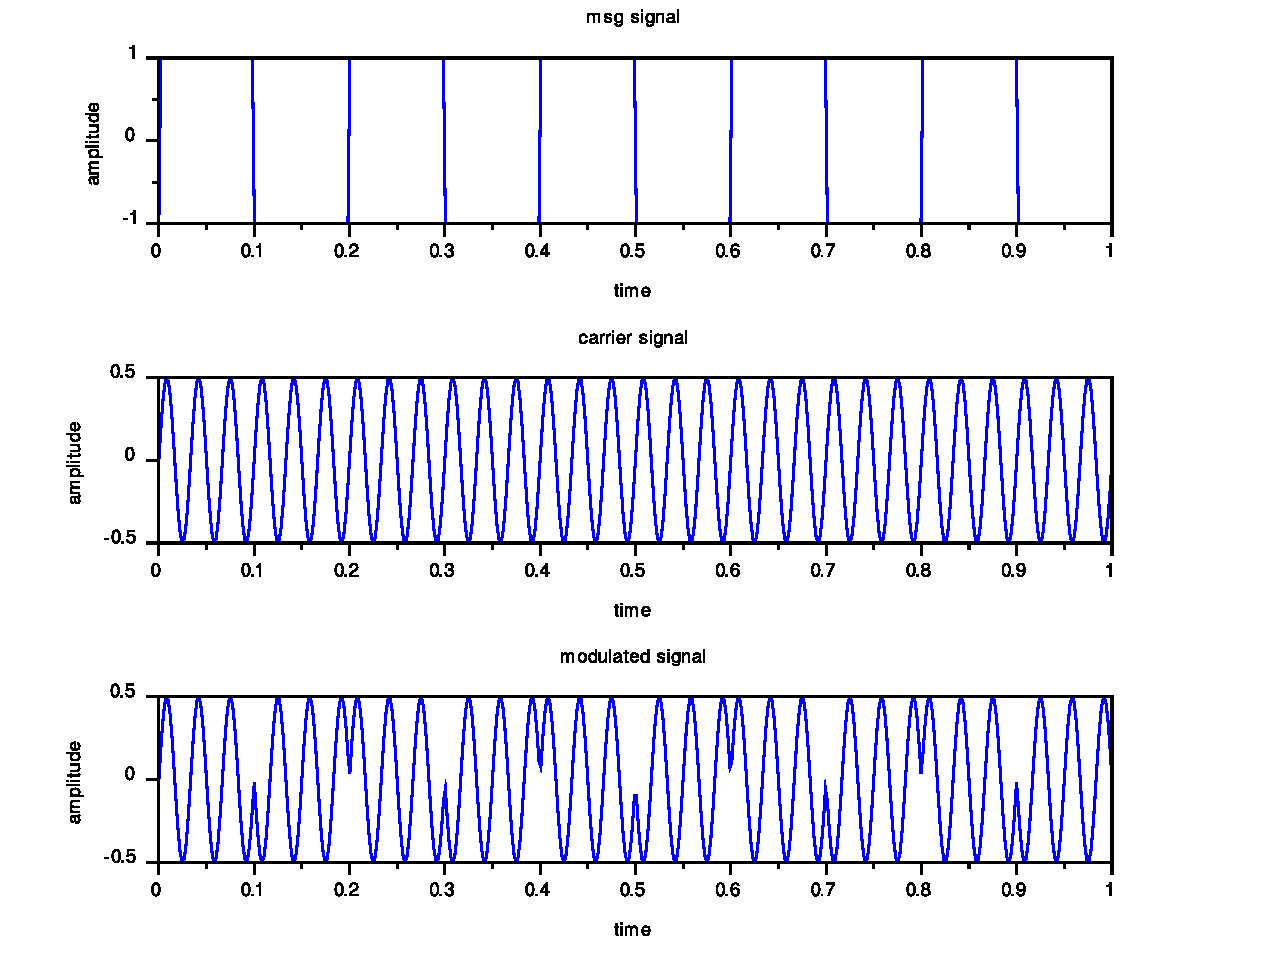
\includegraphics[scale=.7]{/home/kavya/kavyadev/DSPlab/scilabCode/Transmission.pdf}
\caption{Plot of message signal, carrier and BPSK}
\label{transmission}
\end{figure}


\begin{figure}
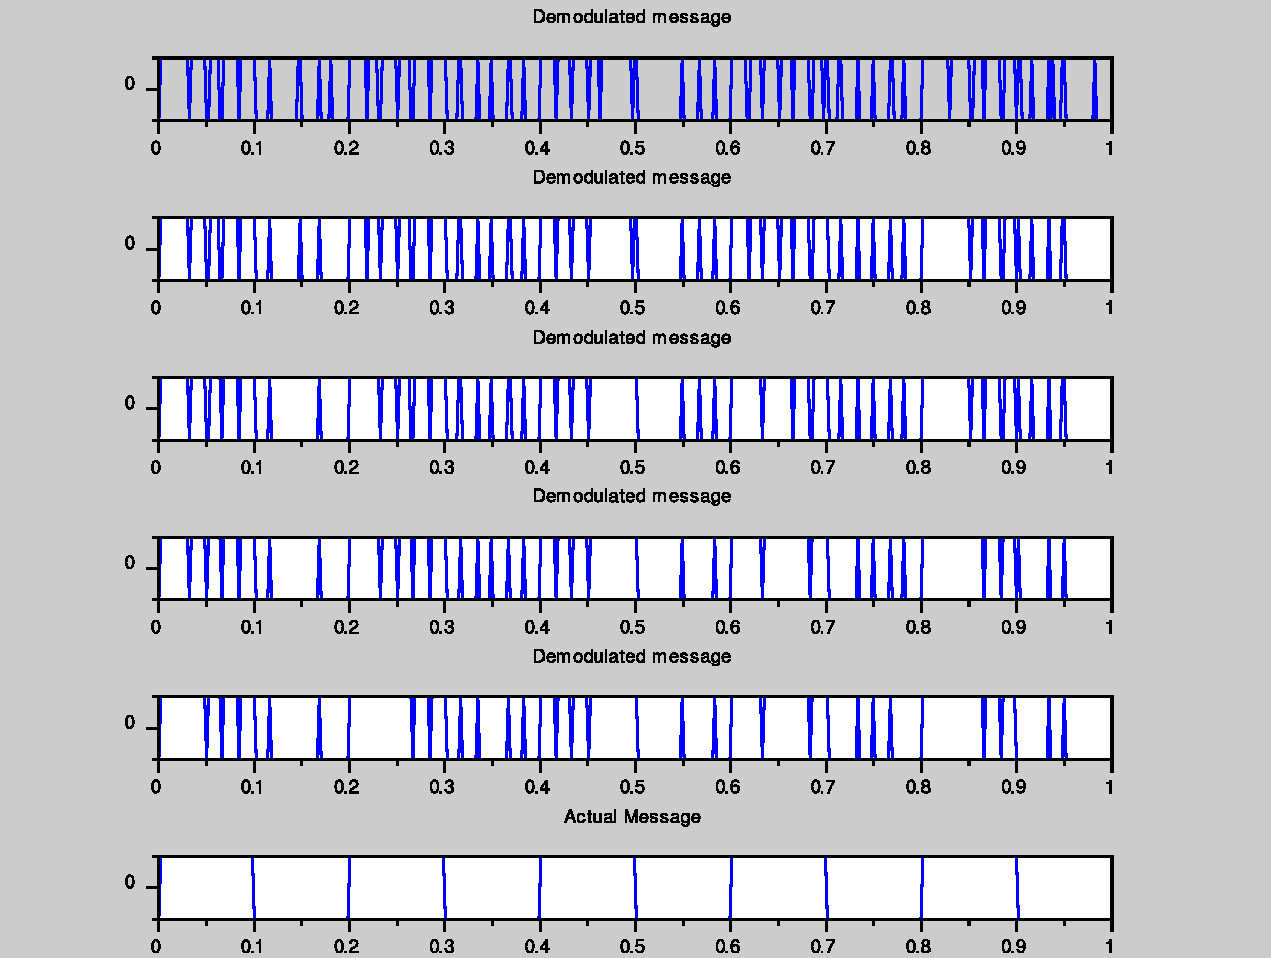
\includegraphics[width=\textwidth, height=15cm]{/home/kavya/kavyadev/DSPlab/scilabCode/Reception.pdf}
\caption{Plot of demodulated signals corresponding to different SNR}
\label{reception}
\end{figure}


\begin{figure}
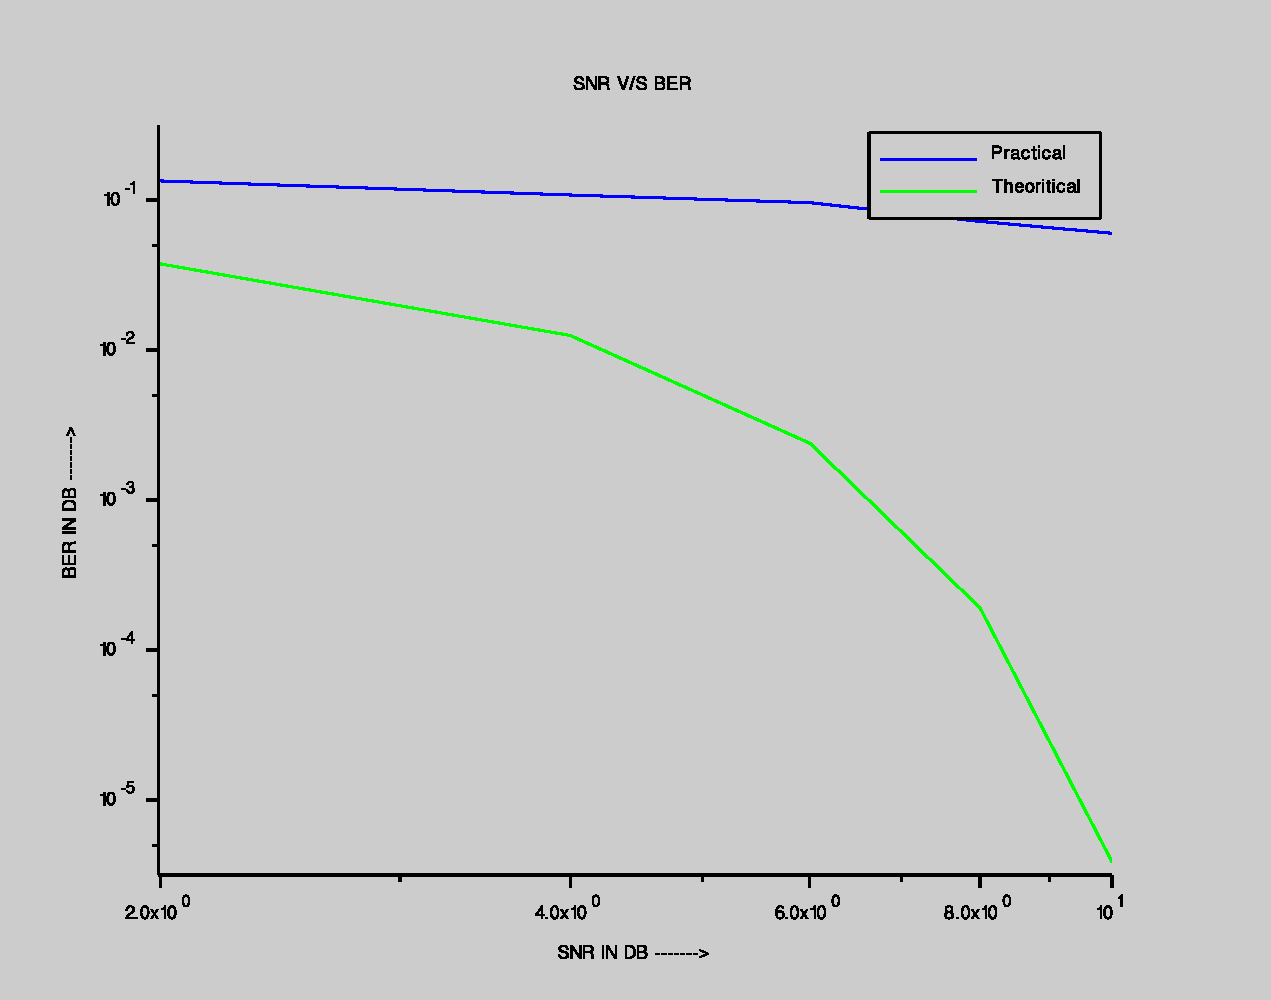
\includegraphics[scale=.7]{/home/kavya/kavyadev/DSPlab/scilabCode/BERVsSNR.pdf}
\caption{Plot of BER Vs SNR (Theoretical and Simulated)}
\label{BER Vs SNR}
\end{figure}

\chapter [Performance Comparison of Modulation Scheme-BASK]{Performance Evaluation of Modulation Scheme-BASK}


\section{AIM}

Implement a digital modulation scheme (BASK) using Scilab. Add noise of different SNR level to model a transmission channel. Demodulate it and find BER for each case and plot it. Compare it with theoretical model.


\section{THEORY}

Digital data with binary values are modulated and represented as the binary amplitude of a sinusoidal carrier in BASK signalling scheme. The decoding will be erroneous if additive noise disrupts the modulated signal during transmission. The bit error rate (BER) decreases with increase in Signal to Noise Ratio (SNR). 

The following experiment compares the theoretical relation between the two with simulated values of BER. Noise corresponding to different values of SNR is added to the modulated signal and the resulting signal is used for message detection. The demodulated message is then compared with the actual message to find the BER corresponding to each value of SNR(2 dB, 4 dB, 6 dB, 8 dB, 10 dB).

\section{PROCEDURE}

\paragraph{}
\begin{enumerate}
\item
Start Scilab on PC and Scilab console window opens. Create a new blank SciNote.
\item
The code for the required program is typed and saved as Scilab SCE file with an extension .sci
\item

The continuous plots are made using the function $plot$ and discrete plots are made using the function $plot2d3$ with the corresponding x axis and y axis variables written inside paranthesis.

\item
To view all the plots in the same window the function $subplot$ is used.
\item
The results and the errors in the program are displayed in the console window.
\item
Figures in every figure window is plotted using $xs2pdf$ function.
The typed program is run using the “execute”.
\end{enumerate}

\section{SCILAB CODE}

\subsection*{Comparison of BER performance for different SNR levels for BASK}
\lstinputlisting[caption=Comparison of BER performance for different SNR levels for BASK]{./scilabCode/berbask.sci}



\section{RESULT}
Performance evaluation plots were implemented.

\begin{figure}
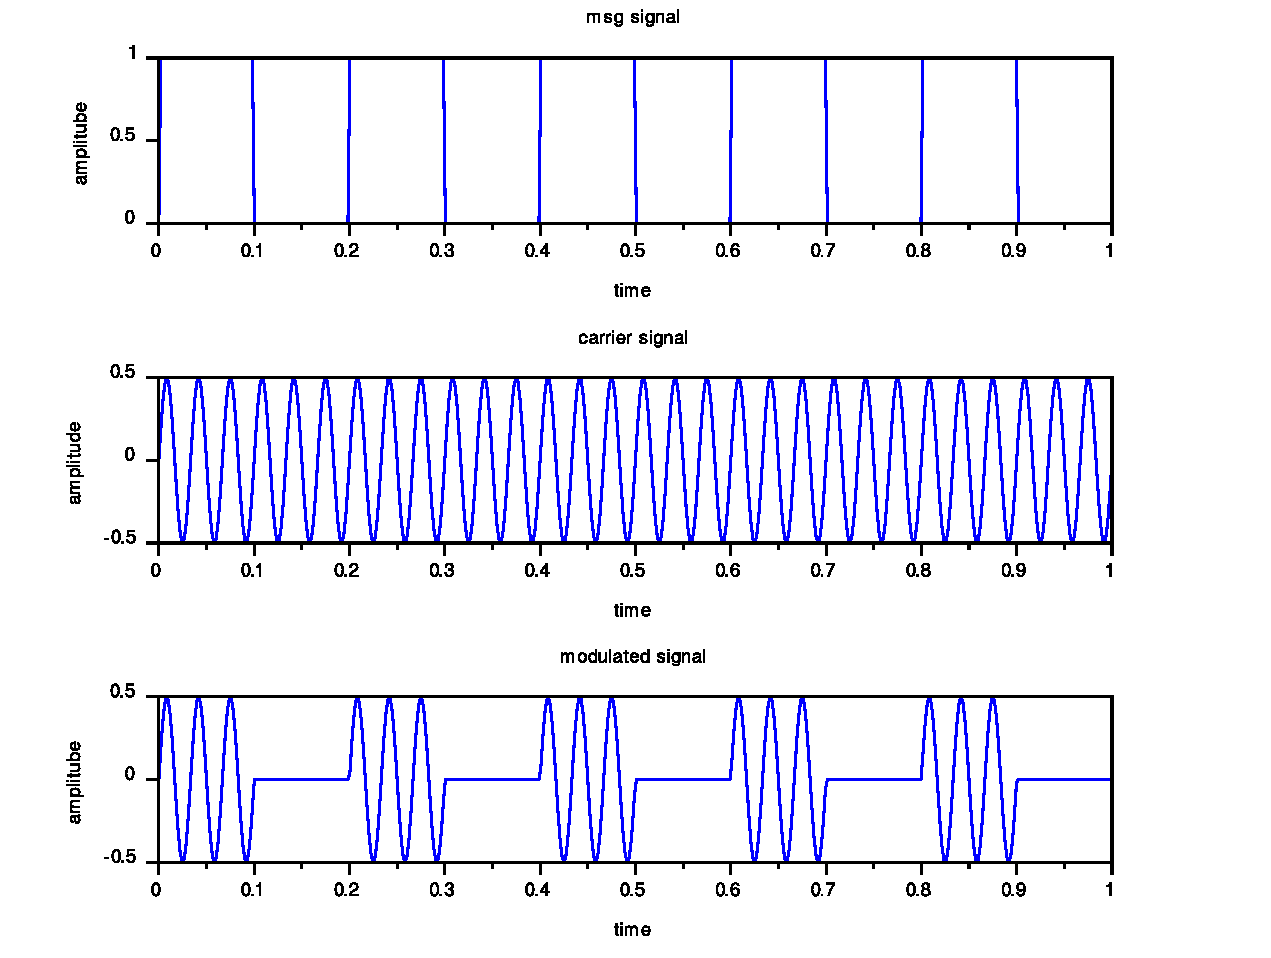
\includegraphics[scale=.7]{/home/kavya/kavyadev/DSPlab/scilabCode/TransmissionASK.pdf}
\caption{Plot of message signal, carrier and BASK}
\label{transmissionask}
\end{figure}


\begin{figure}
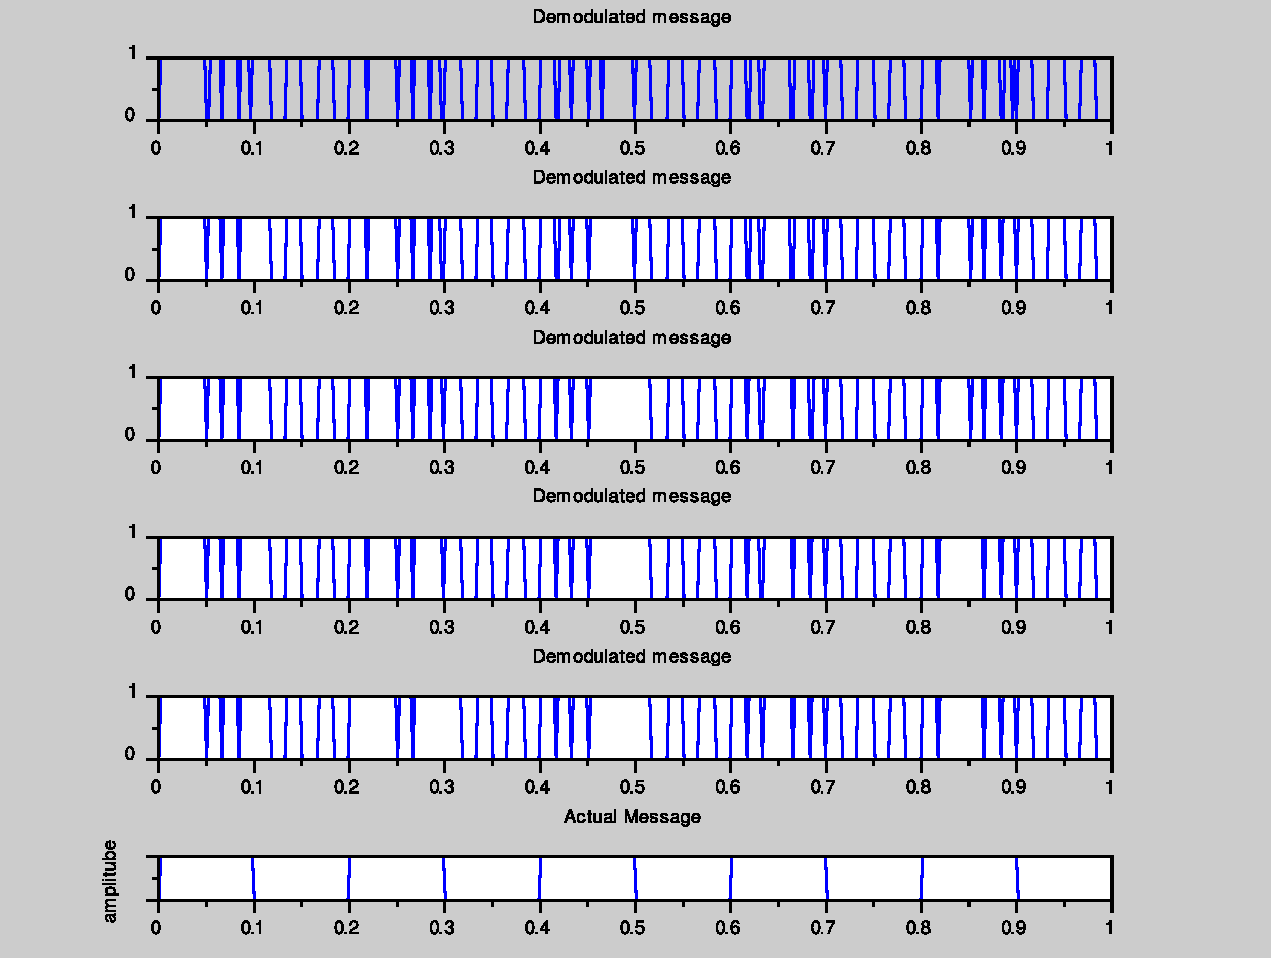
\includegraphics[width=\textwidth, height=15cm]{/home/kavya/kavyadev/DSPlab/scilabCode/ReceptionASK.pdf}
\caption{Plot of demodulated signals corresponding to different SNR}
\label{receptionask}
\end{figure}


\begin{figure}
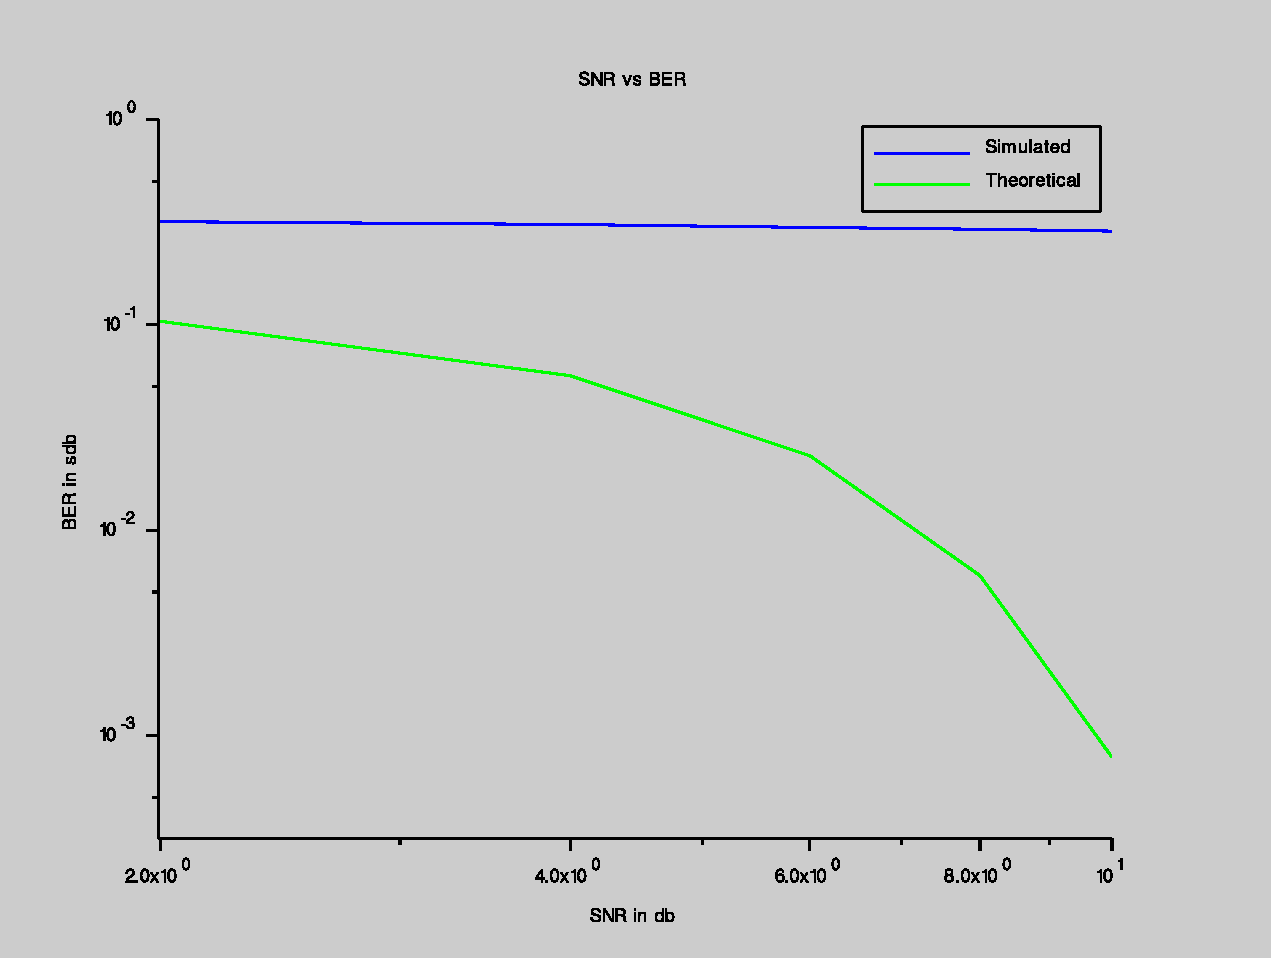
\includegraphics[scale=.7]{/home/kavya/kavyadev/DSPlab/scilabCode/BERVsSNRASK.pdf}
\caption{Plot of BER Vs SNR (Theoretical and Simulated)}
\label{BER Vs SNR}
\end{figure}

%\input{chapters/iir.tex}
%\input{chapters/fir.tex}
%\VerbatimInput{sin.sci}





%\begin{appendix}
%\input{chapters/referencedata.tex}
%\end{appendix}
\begin{thebibliography}{1}

\bibitem{scilab}{\href{http://www.scilab.org/}{Scilab Official Website}}

\bibitem{tutorial}{\href{https://www.cse.iitb.ac.in/~cs626-449/scilab.pdf}{Scilab Tutorial}}

\end{thebibliography}


\end{document}
